\documentclass[12pt, oneside, titlepage]{article}   	% use "amsart" instead of "article" for AMSLaTeX format
\usepackage{geometry}                		% See geometry.pdf to learn the layout options. There are lots.
\geometry{letterpaper}                   		% ... or a4paper or a5paper or ... 
%\geometry{landscape}                		% Activate for rotated page geometry
%\usepackage[parfill]{parskip}    		% Activate to begin paragraphs with an empty line rather than an indent
\usepackage{graphicx}				% Use pdf, png, jpg, or eps§ with pdflatex; use eps in DVI mode
\usepackage{float}                                     % for controlling position of figures in specified location
\usepackage{amssymb}                              % TeX will automatically convert eps --> pdf in pdflatex	
\usepackage[labelfont=bf]{caption}             % make Figure x.x bold

%SetFonts

%SetFonts


\title{\textbf{Documentation of DEMENTpy v1.0}}
\author{Dr. Bin Wang\\Department of Ecology and Evolutionary Biology\\University of California Irvine\\bwang7@uci.edu}
\date{November 1st, 2019}

\begin{document}
\maketitle

\section{Structure}
DEMENTpy is a spatially explicit, trait- and individual-based microbial model that is built from the bottom up from gene all the way up through community to system-level emergent functions.  

% insert a figure here
\begin{figure}[H]
  \centering
  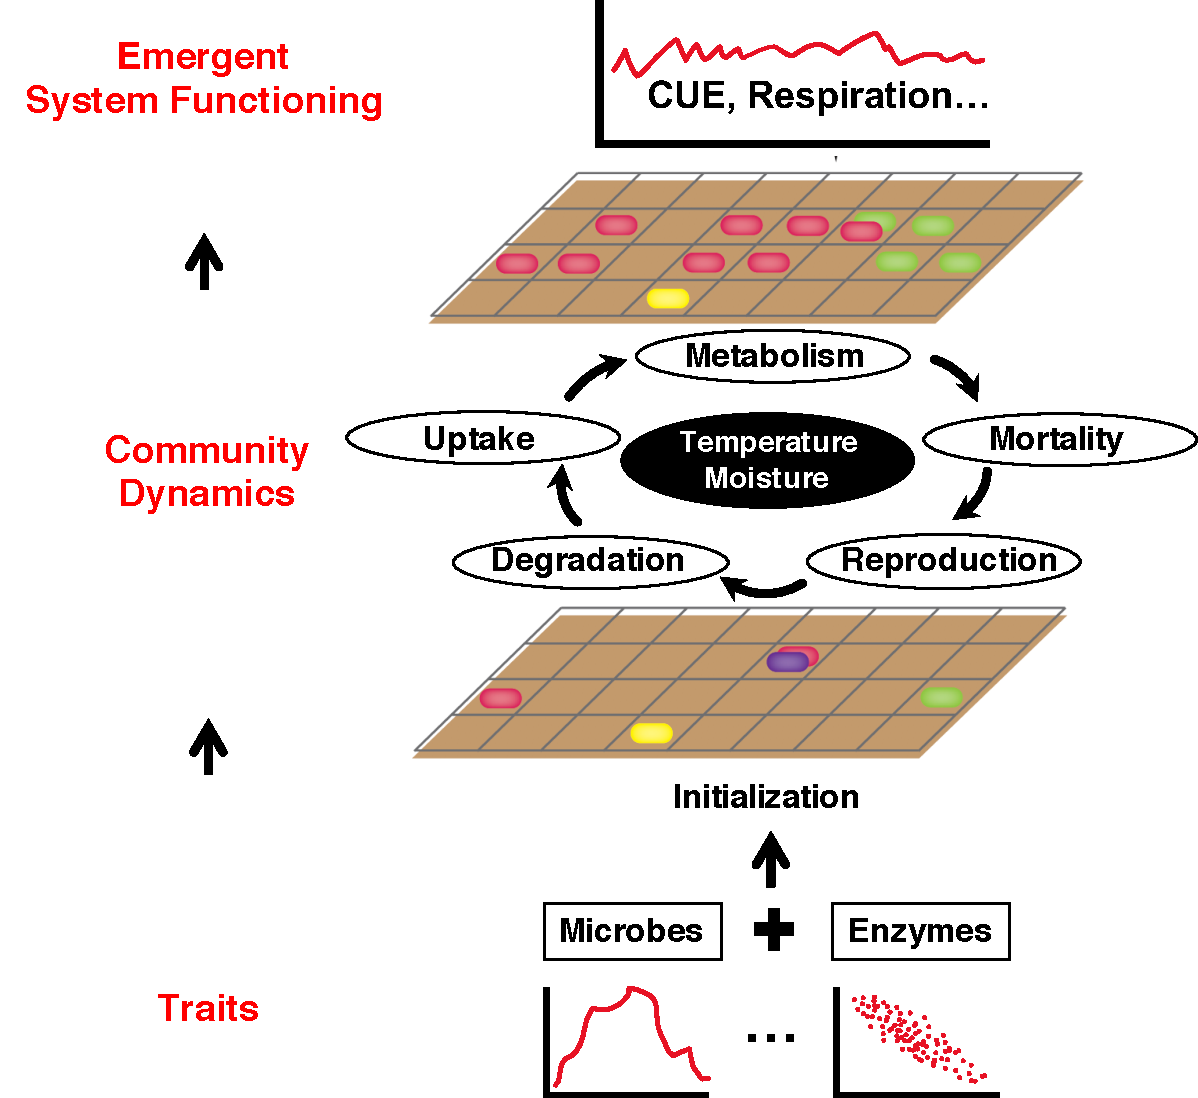
\includegraphics[width=\linewidth]{Fig1_Structure.pdf}
  \caption{DEMENTpy Structure from traits through community to system-level emergent processes.}
  \label{fig:structure}
\end{figure}

\subsection{Modelling Unit}
% insert an illustration of model unit--an individual of a taxon
The modelling unit in DEMENTpy is an individual taxon, which is illustrated as below:


\section{Community Initialization}




\section{Processes}
DEMENTpy is mechanistically explicit model that simulates processes including degradation, uptake, metabolism, mortality, and reproduction. These processes are introduced as below.

\subsection{Degradation}

\subsection{Uptake}

\subsection{Metabolism}

DEMENTpy now explicitly calculates metabolic production of transporters, enzymes, and osmolytes. However, it is noteworthy that for each of these three categories, it is still far from being explicit, especially for osmolyte, which, though it is assumed to have differing genes within each individual taxon and among different taxa, has constant stoichiometry without knowing specific osmotic compounds.

As regards enzyme, different taxa produce different enzymes that have differing kinetic parameters. These different enzymes still have the same stoichiometry, but entail differing metabolic costs for production by different taxa. 

Similar to enzyme, ...

\subsection{Mortality}
Mortality is implemented in DEMENTpy as both a deterministic and a stochastic process. Firstly, a microbial cell dies when its mass reaches a threshold value. In the current version of DEMENTpy the threshold value is assumed to be a constant among taxa. In addition, microbial cells die from a stochastic process, which is, atop a basal mortality probability (differentiated between bacteria and fungi), constrained by drought intensity and drought tolerance, and functional group. These two processes are executed with the deterministic process preceding the stochastic one. The mortality probability is calculated following:

Parameters involved in this mortality process include:

% insert a figure here
\begin{figure}[H]
  \centering
  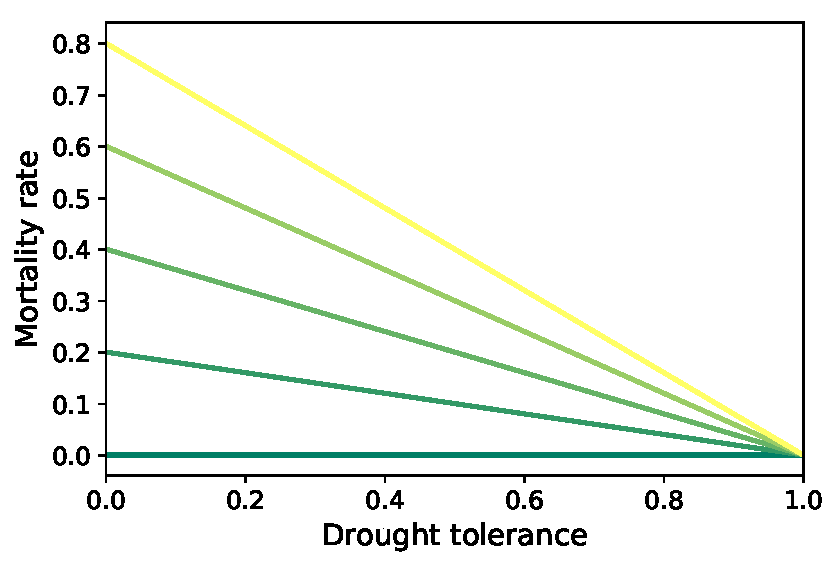
\includegraphics[width=\linewidth]{Fig2_Microbial_mortality_prob.pdf}
  \caption{Microbial mortality as a function of drought and tolerance.}
  \label{fig:mortality}
\end{figure}


\subsection{Reproduction}
-
-



\section{Simulation Protocol}
--

\section{DEMENTpy Programming Structure}

% insert the diagram of structure

\section{Running DEMENTpy}

DEMENTpy is open source project, of which the code is archived on GitHub at: https://github.com/bioatmosphere/DEMENTpy.


\end{document}  